% =============================================================
% Codebook 主檔說明
% - 目標：在最少頁數內排入常用演算法 / 資料結構程式碼。
% - 版面：使用 twocolumn 壓縮，手動設定窄邊界，字體縮小。
% - 編譯：建議使用 xelatex (需支援 fontspec / xeCJK)。
% - 可調整項目：行號 (listings)、字型、是否加入更多章節。
% =============================================================
\documentclass[a4paper,10pt,twocolumn,oneside]{article}
\setlength{\columnsep}{10pt}                                                              %兩欄模式的間距
\setlength{\columnseprule}{0pt}                                                                %兩欄模式間格線粗細

\usepackage{amsthm}								%定義，例題
\usepackage{amssymb}
%\usepackage[margin=2cm]{geometry}
\usepackage{fontspec}								%設定字體
\usepackage{color}
\usepackage[x11names]{xcolor}
\usepackage{listings}								%顯示code用的
%\usepackage[Glenn]{fncychap}						%排版，頁面模板
\usepackage{fancyhdr}								%設定頁首頁尾
\usepackage{graphicx}								%Graphic
\usepackage{enumerate}
\usepackage{titlesec}
\usepackage{amsmath}
\usepackage{tikz}
\usepackage{xpatch}
\usepackage[CheckSingle, CJKmath]{xeCJK}
% \usepackage{CJKulem}
%\usepackage[T1]{fontenc}
\titlespacing{\section}{0cm}{0cm}{0cm}
\titlespacing{\subsection}{0cm}{0cm}{0cm}
\usepackage{amsmath, courier, listings, fancyhdr, graphicx}
\topmargin=0pt
\headsep=5pt
\textheight=780pt
\footskip=0pt
\voffset=-40pt
\textwidth=545pt
\marginparsep=0pt
\marginparwidth=0pt
\marginparpush=0pt
\oddsidemargin=0pt
\evensidemargin=0pt
\hoffset=-42pt

%\renewcommand\listfigurename{圖目錄}
%\renewcommand\listtablename{表目錄} 

%%%%%%%%%%%%%%%%%%%%%%%%%%%%%


\setmainfont [				%主要字型
    Path = .fonts/ttf/,
    UprightFont = *-Regular,
    BoldFont = *-Bold,
    ItalicFont = *-Italic
  ] {Consolas}

\setmonofont [        
    Path = .fonts/ttf/,
    UprightFont = *-Regular
  ] {Monaco}

\setCJKmainfont[
  Path = .fonts/ttf/,        % 你放字型檔的資料夾（相對於主 .tex 檔案）
  Extension = .ttf,
  UprightFont = *-Regular,
  BoldFont = *-Bold,
]{NotoSansTC}

\XeTeXlinebreaklocale "zh"						%中文自動換行
\XeTeXlinebreakskip = 0pt plus 1pt				%設定段落之間的距離
\setcounter{secnumdepth}{3}						%目錄顯示第三層

%%%%%%%%%%%%%%%%%%%%%%%%%%%%%
\makeatletter
\lst@CCPutMacro\lst@ProcessOther {"2D}{\lst@ttfamily{-{}}{-{}}}
\@empty\z@\@empty
\makeatother
\lstset{											% Code顯示
language=C++,										% the language of the code
basicstyle=\footnotesize\ttfamily, 						% the size of the fonts that are used for the code
%numbers=left,										% where to put the line-numbers
numberstyle=\footnotesize,						% the size of the fonts that are used for the line-numbers
stepnumber=1,										% the step between two line-numbers. If it's 1, each line  will be numbered
numbersep=5pt,										% how far the line-numbers are from the code
backgroundcolor=\color{white},					% choose the background color. You must add \usepackage{color}
showspaces=false,									% show spaces adding particular underscores
showstringspaces=false,							% underline spaces within strings
showtabs=false,									% show tabs within strings adding particular underscores
frame=false,											% adds a frame around the code
tabsize=2,											% sets default tabsize to 2 spaces
captionpos=b,										% sets the caption-position to bottom
breaklines=true,									% sets automatic line breaking
breakatwhitespace=false,							% sets if automatic breaks should only happen at whitespace
escapeinside={\%*}{*)},							% if you want to add a comment within your code
morekeywords={*},									% if you want to add more keywords to the set
keywordstyle=\bfseries\color{Blue1},
commentstyle=\itshape\color{Red4},
stringstyle=\itshape\color{Green4},
}

%%%%%%%%%%%%%%%%%%%%%%%%%%%%%

\begin{document}
\pagestyle{fancy}
\fancyfoot{}
%\fancyfoot[R]{\includegraphics[width=20pt]{ironwood.jpg}}
\fancyhead[L]{Jackis666}
\fancyhead[R]{\thepage}
\renewcommand{\headrulewidth}{0.4pt}
\renewcommand{\contentsname}{Contents} 

\newcommand{\includetex}[2]{
  \subsection{#1}
  \input{#2}
  \vspace{-1.2em}
}
\scriptsize
\tableofcontents


% \newpage
%sectionstart  % ===== 以下依分類匯入各程式碼檔案 =====

\section{Basic}
    \subsection{default}
    \lstinputlisting{basic/default.cpp}

    \subsection{奇妙的東西}
    \lstinputlisting{basic/coolthings.cpp}

    \subsection{random}
    \lstinputlisting{basic/random.cpp}

%====================================================

\section{Math}
  \subsection{basic}
  \lstinputlisting{math/basic}

  \subsection{快速幂}
  \lstinputlisting{math/pow.cpp}

  \subsection{大數運算}
  \lstinputlisting{math/bigmath.cpp}

  \subsection{極座標排序}
  \lstinputlisting{math/sort_of_point.cpp}

  \includetex{Theorem}{math/theorem}
  \vspace{1.2em}

  \includetex{Prime}{math/prime.tex}
  \vspace{1.2em}

%====================================================

\section{Binary Search}
    \subsection{二分搜}
    \lstinputlisting{binary search/binary search.cpp}

    \subsection{三分搜}
    \lstinputlisting{binary search/tenary search.cpp}

%====================================================

\section{DataStructure}
    \subsection{DSU(並查集)}
    \lstinputlisting{datastructure/dsu.cpp}
    
    \subsection{FenwickTree/BIT}
    \lstinputlisting{datastructure/BIT.cpp}

    \subsection{Seg}
    \lstinputlisting{datastructure/Seg.cpp}

%====================================================

\section{Graph}
    \subsection{Topo/拓樸}
    \lstinputlisting{graph/topo.cpp}


%====================================================

\newcommand{\halfgridpage}{
    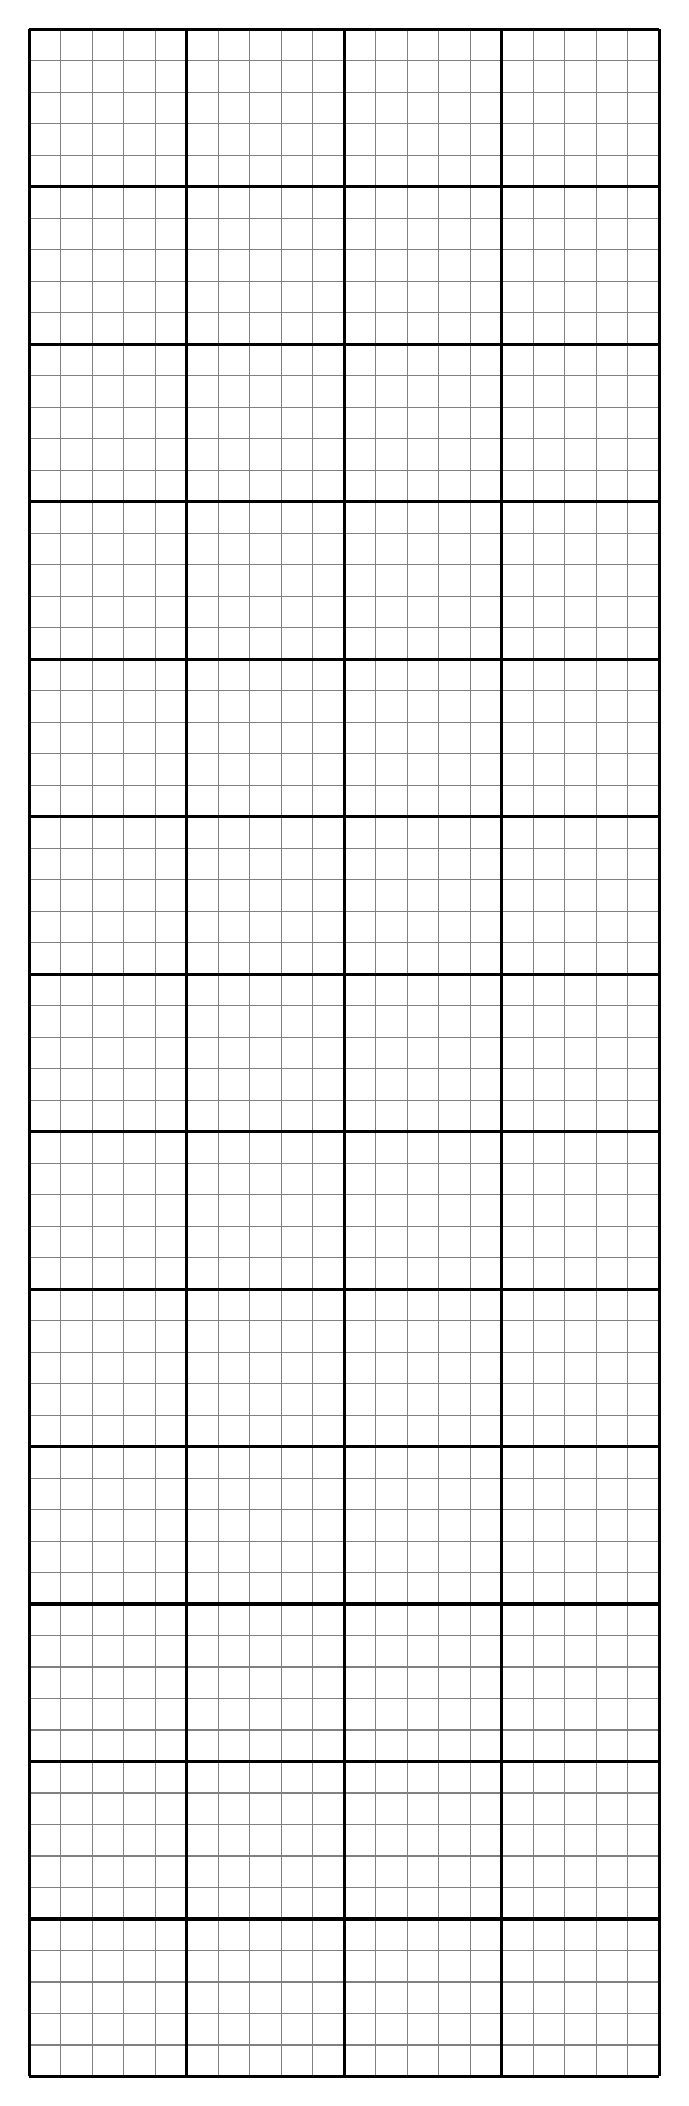
\begin{tikzpicture}[every node/.style={minimum size=1cm-\pgflinewidth, outer sep=10pt}, scale=2]
        \draw[step=0.2cm,color=gray] (0,0) grid (4,13);
        \draw[step=1cm,color=black,line width=0.4mm] (0,0) grid (4,13);
    \end{tikzpicture}
    \newpage
}
\newcommand{\gridpage}{
    \centering
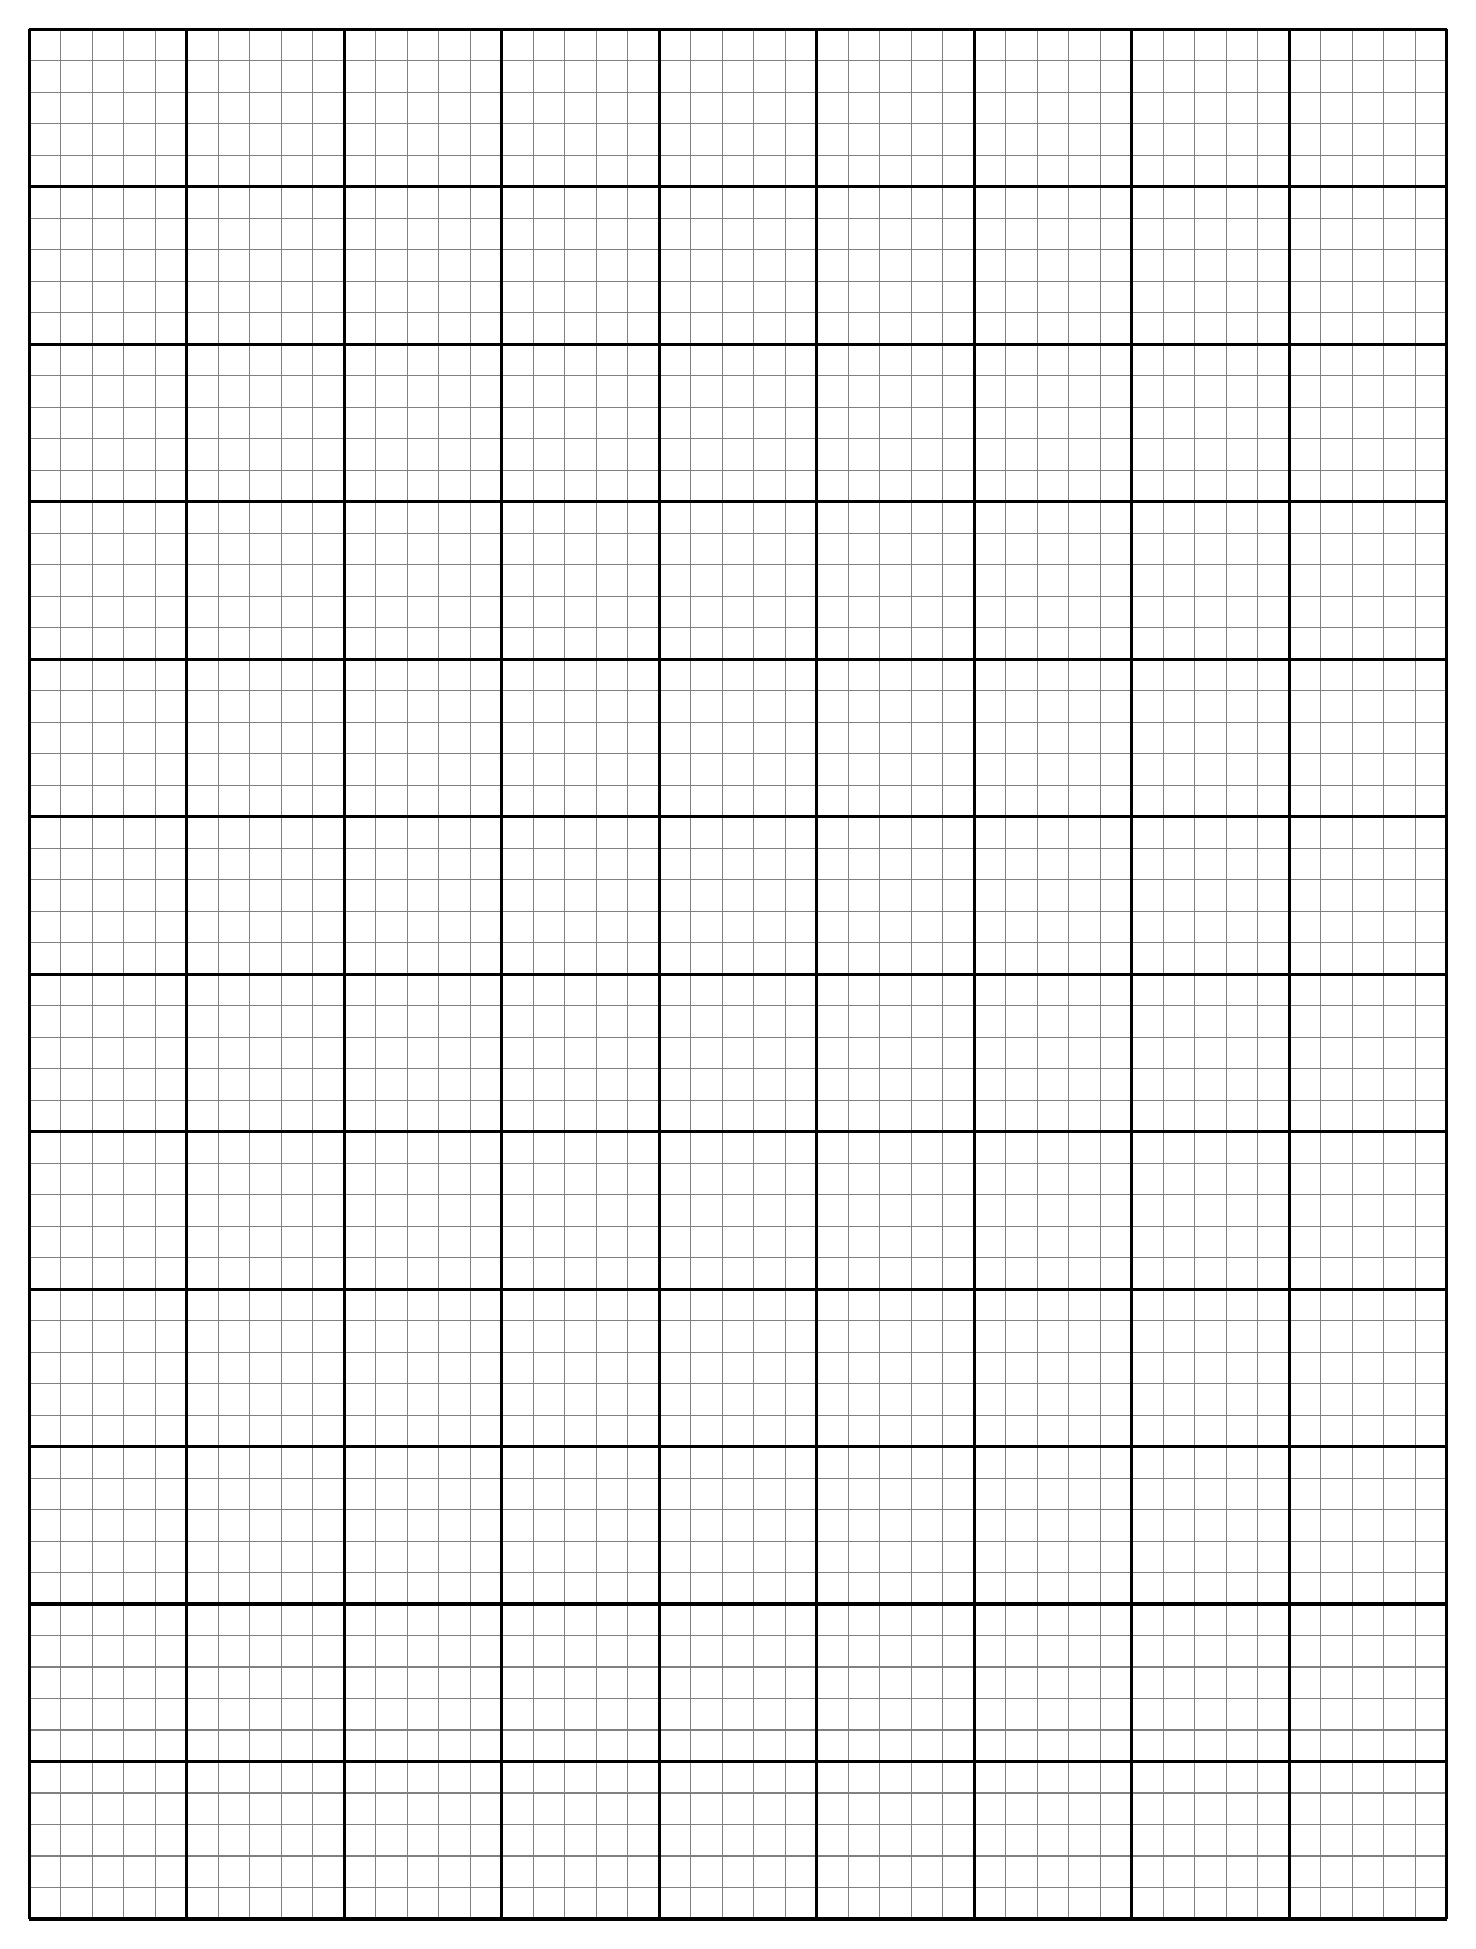
\begin{tikzpicture}[every node/.style={minimum size=1cm-\pgflinewidth, outer sep=10pt}, scale=2]
    \draw[step=0.2cm,color=gray] (0,0) grid (9,12);
    \draw[step=1cm,color=black,line width=0.4mm] (0,0) grid (9,12);
\end{tikzpicture}
    \newpage
}
\onecolumn
\gridpage
\gridpage
\gridpage
\gridpage


\end{document}